%  LaTeX support: latex@mdpi.com 
%  In case you need support, please attach all files that are necessary for compiling as well as the log file, and specify the details of your LaTeX setup (which operating system and LaTeX version / tools you are using).

% You need to save the "mdpi.cls" and "mdpi.bst" files into the same folder as this template file.

%=================================================================
\documentclass[jof,article,submit,moreauthors,pdftex,10pt,a4paper]{Definitions/mdpi} 

% If you would like to post an early version of this manuscript as a preprint, you may use preprint as the journal and change 'submit' to 'accept'. The document class line would be, e.g., \documentclass[preprints,article,accept,moreauthors,pdftex,10pt,a4paper]{mdpi}. This is especially recommended for submission to arXiv, where line numbers should be removed before posting. For preprints.org, the editorial staff will make this change immediately prior to posting.

%
%--------------------
% Class Options:
%--------------------
% jof
%----------
% Choose between the following MDPI journals:
% acoustics, actuators, addictions, admsci, aerospace, agriculture, agronomy, algorithms, animals, antibiotics, antibodies, antioxidants, applsci, arts, asi, atmosphere, atoms, axioms, batteries, bdcc, behavsci, beverages, bioengineering, biology, biomedicines, biomimetics, biomolecules, biosensors, brainsci, buildings, carbon, cancers, catalysts, cells, ceramics, challenges, chemengineering, chemosensors, children, cleantechnol, climate, clockssleep, cmd, coatings, colloids, computation, computers, condensedmatter, cosmetics, cryptography, crystals, cybersecurity, data, dentistry, designs, diagnostics, dairy, diseases, diversity, drones, econometrics, economies, education, electrochem, electrochemistry, electronics, energies, entropy, environments, epigenomes, est, fermentation, fibers, fire, fishes, fluids, foods, forecasting, forests, fractalfract, futureinternet, galaxies, games, gastrointestdisord, gels, genealogy, genes, geohazards, geosciences, geriatrics, hazardousmatters, healthcare, heritage, highthroughput, horticulturae, humanities, hydrology, informatics, information, infrastructures, inorganics, insects, instruments, ijerph, ijfs, ijms, ijgi, ijtpp, inventions, j, jcdd, jcm, jcs, jdb, jfb, jfmk, jimaging, jof, jintelligence, jlpea, jmmp, jmse, jpm, jrfm, jsan, land, languages, laws, life, literature, logistics, lubricants, machines, magnetochemistry, make, marinedrugs, materials, mathematics, mca, medsci, medicina, medicines, membranes, metabolites, metals, microarrays, micromachines, microorganisms, minerals, modelling, molbank, molecules, mps, mti, nanomaterials, ncrna, neonatalscreening, neuroglia, nitrogen, nutrients, ohbm, particles, pathogens, pharmaceuticals, pharmaceutics, pharmacy, philosophies, photonics, plants, plasma, polymers, polysaccharides, proceedings, processes, proteomes, publications, quaternary, qubs, reactions, recycling, religions, remotesensing, reports, resources, risks, robotics, safety, sci, scipharm, sensors, separations, sexes, sinusitis, smartcities, socsci, societies, soilsystems, sports, standards, stats, surfaces, surgeries, sustainability, symmetry, systems, technologies, toxics, toxins, tropicalmed, universe, urbansci, vaccines, vehicles, vetsci, vibration, viruses, vision, water, wem, wevj
%---------
% article
%---------
% The default type of manuscript is article, but can be replaced by: 
% abstract, addendum, article, benchmark, book, bookreview, briefreport, casereport, changes, comment, commentary, communication, conceptpaper, correction, conferenceproceedings, conferencereport, expressionofconcern, extendedabstract, meetingreport, creative, datadescriptor, discussion, editorial, essay, erratum, hypothesis, interestingimages, letter, meetingreport, newbookreceived, opinion, obituary, projectreport, reply, reprint, retraction, review, perspective, protocol, shortnote, supfile, technicalnote, viewpoint
% supfile = supplementary materials
% protocol: If you are preparing a "Protocol" paper, please refer to http://www.mdpi.com/journal/mps/instructions for details on its expected structure and content.
%----------
% submit
%----------
% The class option "submit" will be changed to "accept" by the Editorial Office when the paper is accepted. This will only make changes to the frontpage (e.g., the logo of the journal will get visible), the headings, and the copyright information. Also, line numbering will be removed. Journal info and pagination for accepted papers will also be assigned by the Editorial Office.
%------------------
% moreauthors
%------------------
% If there is only one author the class option oneauthor should be used. Otherwise use the class option moreauthors.
%---------
% pdftex
%---------
% The option pdftex is for use with pdfLaTeX. If eps figures are used, remove the option pdftex and use LaTeX and dvi2pdf.

%\usepackage{biblatex}
%\addbibresource{mendeley_v2.bib}
\newcommand{\textlower}{$<$}
\newcommand{\TODO}[1]{\textbf{\color{red}{#1}}}
\newcommand{\exoDer}{\textit{Exophiala dermatitidis}}
\newcommand{\exoMes}{\textit{Exophiala mesophila}}
\newcommand{\exoSid}{\textit{Exophiala sideris}}
\newcommand{\exoSpi}{\textit{Exophiala spinifera}}
\newcommand{\claImm}{\textit{Cladophialophora immunda}}
\newcommand{\fonPed}{\textit{Fonsacaea pedrosi}}
\newcommand{\horWer}{\textit{Hortea werneckii}}
\newcommand{\canAlb}{\textit{Candida albicans}}
\newcommand{\aspNig}{\textit{Aspergillus niger}}
\newcommand{\aspNid}{\textit{Aspergillus nidulans}}
\newcommand{\aspFum}{\textit{Aspergillus fumigatus}}
\newcommand{\aspRub}{\textit{Aspergillus ruber}}
\newcommand{\penChr}{\textit{Penicillium chrysogenum}}
\newcommand{\debFab}{\textit{Debaryomyces fabryi}}
\newcommand{\debHan}{\textit{Debaryomyces hansenii}}
\newcommand{\walIch}{\textit{Walemia ichthyophaga}}
\newcommand{\walMel}{\textit{Walemia mellicola}}
\newcommand{\canPar}{\textit{Candida parapsilosis}}
\newcommand{\cocImm}{\textit{Coccidioides immitis}}
\newcommand{\triRub}{\textit{Trichophyton rubrum}}
\newcommand{\thiTer}{\textit{Thielavia terrestris}}
\newcommand{\mycThe}{\textit{Myceliophthora thermophila}}
\newcommand{\neuCra}{\textit{Neurospora crassa}}
\newcommand{\sacCer}{\textit{Saccharomyces cerevisiae}}
\newcommand{\schPom}{\textit{Schizosaccharomyces pombe}}
\newcommand{\cryNeo}{\textit{Cryptococcus neoformans}}
\newcommand{\micCan}{\textit{Microsporum canis}}
\newcommand{\onyCor}{\textit{Onygena corvina}}
\newcommand{\blaDer}{\textit{Blastomyces dermatitidis}}
\newcommand{\parBra}{\textit{Paracoccidioides brasiliensis}}
\newcommand{\cocPos}{\textit{Coccidioides posadasii}}
\newcommand{\toxGon}{\textit{Toxoplasma gondii}}
\newcommand{\fusOxy}{\textit{Fusarium oxysporum}}
\newcommand{\fusSol}{\textit{Fusarium solani}}
\newcommand{\tryRub}{\textit{Fusarium solani}}
\newcommand{\clado}{\textit{Cladophialophora}}
\newcommand{\attspe}{\textit{Attalea speciosa}}
\newcommand{\claban}{\textit{Cladophialophora bantiana}}
\newcommand{\clasat}{\textit{Cladophialophora saturnica}}
\newcommand{\clapsa}{\textit{Cladophialophora psammophila}}
\newcommand{\clasph}{\textit{Cladosporium sphaerospermum}}
\newcommand{\claBan}{\textit{Cladophialophora bantiana}}
\newcommand{\fusGra}{\textit{Fusarium graminearum}}
\newcommand{\fusSpo}{\textit{Fusarium sporotrichoides}}
\newcommand{\triAru}{\textit{Trichoderma arundinaceum}}
\newcommand{\triBre}{\textit{Trichoderma brevicompactum}}
\newcommand{\phiSp}{\textit{Aspergillus salisburgensis}}
\newcommand{\phiScl}{\textit{Aspergillus sclerolatus}}
\newcommand{\staCha}{\textit{Stachybotrys chartarum}}
\newcommand{\staChl}{\textit{Stachybotrys chloronata}}
\newcommand{\ustMay}{\textit{Ustilago maydis}}
\newcommand{\exo}{\textit{Exophiala}}
\newcommand{\herpo}{\textit{Herpotrichiellaceae}}
\newcommand{\skin}{skin}
\newcommand{\tol}{\textit{toluene}}
\newcommand{\glu}{\textit{glucose}}

%=================================================================
\firstpage{1} 
\makeatletter 
\setcounter{page}{\@firstpage} 
\makeatother
\pubvolume{xx}
\issuenum{1}
\articlenumber{5}
\pubyear{2018}
\copyrightyear{2018}
%\externaleditor{Academic Editor: name}
\history{Received: date; Accepted: date; Published: date}
%\updates{yes} % If there is an update available, un-comment this line

%% MDPI internal command: uncomment if new journal that already uses continuous page numbers 
%\continuouspages{yes}

%------------------------------------------------------------------
% The following line should be uncommented if the LaTeX file is uploaded to arXiv.org
%\pdfoutput=1

%=================================================================
% Add packages and commands here. The following packages are loaded in our class file: fontenc, calc, indentfirst, fancyhdr, graphicx, lastpage, ifthen, lineno, float, amsmath, setspace, enumitem, mathpazo, booktabs, titlesec, etoolbox, amsthm, hyphenat, natbib, hyperref, footmisc, geometry, caption, url, mdframed, tabto, soul, multirow, microtype, tikz

%=================================================================
%% Please use the following mathematics environments: Theorem, Lemma, Corollary, Proposition, Characterization, Property, Problem, Example, ExamplesandDefinitions, Hypothesis, Remark, Definition
%% For proofs, please use the proof environment (the amsthm package is loaded by the MDPI class).

%=================================================================
% Full title of the paper (Capitalized)
\Title{Back to the salt mines: A genome and transcriptome analyses of the halophilic Hallstatt fungus Aspergillus salinarum}

% Author Orchid ID: enter ID or remove command
%\newcommand{\orcidauthorA}{0000-0000-000-000X} % Add \orcidA{} behind the author's name
%\newcommand{\orcidauthorB}{0000-0000-000-000X} % Add \orcidB{} behind the author's name

% Authors, for the paper (add full first names)
\Author{Hakim Tafer $^{1}$, Caroline Poyntner $^{1}$, Ksenija Lopandic $^{1}$, Katja Sterflinger $^{1}$ and Guadalupe Pi\~nar $^{1,*}$}

% Authors, for metadata in PDF
\AuthorNames{Hakim Tafer , Caroline Poyntner , Ksenija Lopandic and Guadalupe Pi\~nar}

% Affiliations / Addresses (Add [1] after \address if there is only one affiliation.)
\address{%
$^{1}$ \quad Extremophiles Center, Department of Biotechnology, University of Natural Resources and Life Sciences Muthgasse 18, 1190 Vienna, Austria\\
% Contact information of the corresponding author
\corres{Correspondence: guadalupe.pinar@boku.ac.at}}

% Current address and/or shared authorship
%\firstnote{Current address: Affiliation 3} 
%\secondnote{These authors contributed equally to this work.}
% The commands \thirdnote{} till \eighthnote{} are available for further notes

%\simplesumm{} % Simple summary

%\conference{} % An extended version of a conference paper

% Abstract (Do not insert blank lines, i.e. \\) 
\abstract{Salt mines are among the most extreme environment as they combine darkness, low nutrient availability and hypersaline conditions. Based on comparative genomics and transcriptomics, we describe in this work the adaptive strategies of the true halophile {\phiSp} found in a salt mine in Austria and compare them to the ex-type halotolerant strain {\phiScl}. On a genomic level, {\phiSp} exhibits a reduced genome size compared to {\phiSp} as well as a contraction of genes involved in transport processes. The proteome of {\phiSp} exhibits an increased proportion of alanine, glycine and proline compared to the proteome of non-halophilic species. Transcriptome analyses of both strains growing at 5$\%$ and 20$\%$ NaCl show that {\phiSp} regulates three times fewer genes than {\phiScl} in order to adapt to the higher salt concentration. In {\phiScl}, the increased osmotic stress impacted processes related to translation, transcription, transport and energy. In contrast, membrane-related proteins were significantly affected in {\phiSp}.}

% Keywords
\keyword{keyword 1; keyword 2; keyword 3 (list three to ten pertinent keywords specific to the article, yet reasonably common within the subject discipline.)}

% The fields PACS, MSC, and JEL may be left empty or commented out if not applicable
%\PACS{J0101}
%\MSC{}
%\JEL{}

%%%%%%%%%%%%%%%%%%%%%%%%%%%%%%%%%%%%%%%%%%
% Only for the journal Diversity
%\LSID{\url{http://}}

%%%%%%%%%%%%%%%%%%%%%%%%%%%%%%%%%%%%%%%%%%
% Only for the journal Applied Sciences:
%\featuredapplication{Authors are encouraged to provide a concise description of the specific application or a potential application of the work. This section is not mandatory.}
%%%%%%%%%%%%%%%%%%%%%%%%%%%%%%%%%%%%%%%%%%

%%%%%%%%%%%%%%%%%%%%%%%%%%%%%%%%%%%%%%%%%%
% Only for the journal Data:
%\dataset{DOI number or link to the deposited data set in cases where the data set is published or set to be published separately. If the data set is submitted and will be published as a supplement to this paper in the journal Data, this field will be filled by the editors of the journal. In this case, please make sure to submit the data set as a supplement when entering your manuscript into our manuscript editorial system.}

%\datasetlicense{license under which the data set is made available (CC0, CC-BY, CC-BY-SA, CC-BY-NC, etc.)}

%%%%%%%%%%%%%%%%%%%%%%%%%%%%%%%%%%%%%%%%%%
% Only for the journal Toxins
%\keycontribution{The breakthroughs or highlights of the manuscript. Authors can write one or two sentences to describe the most important part of the paper.}

%\setcounter{secnumdepth}{4}
%%%%%%%%%%%%%%%%%%%%%%%%%%%%%%%%%%%%%%%%%%
\begin{document}
%%%%%%%%%%%%%%%%%%%%%%%%%%%%%%%%%%%%%%%%%%
%% Only for the journal Gels: Please place the Experimental Section after the Conclusions

%%%%%%%%%%%%%%%%%%%%%%%%%%%%%%%%%%%%%%%%%%
%\setcounter{section}{-1} %% Remove this when starting to work on the template.

%The order of the section titles is: Introduction, Materials and Methods, Results, Discussion, Conclusions for these journals: aerospace,algorithms,antibodies,antioxidants,atmosphere,axioms,biomedicines,carbon,crystals,designs,diagnostics,environments,fermentation,fluids,forests,fractalfract,informatics,information,inventions,jfmk,jrfm,lubricants,neonatalscreening,neuroglia,particles,pharmaceutics,polymers,processes,technologies,viruses,vision

\section{Introduction}
Saline and hypersaline environments like salt marshes, saline soil and water, the Dead Sea are home to a great fungal diversity~\cite{Gunde-Cimerman2014}. The vast majority are either as halotolerant or as extremely halotolerant, i.e. they can grow without NaCl but can also withstand salt concentration up to 30$\%$ ~\cite{Gunde-Cimerman2000}. Halophile fungi, that is fungi that need a given concentration of NaCl in order to survive, are uncommon~\cite{Gunde-Cimerman2000}. Currently only \walIch{}, \textit{Wallemia muriae}, \textit{Aspergillus baarnensis}, \textit{Aspergillus salinarium} and \aspRub{}~\cite{Kis-Papo2014-dn} are classified as halophile. Recently \phiSp{}, a fungus isolated from from historical wooden staircase in a salt mine in Austria~\cite{Martinelli2017AspergillusMorphology} was added to the list of halophile.

The ability to survive osmotic stress requires several adaptation. \walIch whithstand high salt concentration by increasing the intracellular concentration of polyols in order to counteract the increased osmotic pressure, uses high-affinity K$^+$ transporters and thickens its cell-wall by a factor of three~\cite{Zajc2013}. \aspRub under high salt concentration increases the number of ion transporters, exhibit a higher proportion of acidic amino acid, restructures its cell-wall and uses Glycerol as compatible solute~\cite{Kis-Papo2014-dn}.
Similar adaptation strategies are found in halotolerant species where the production of hydrophilic compounds, such as amino acids, sugar alcohols, soluble sugars to achieve osmotic equilibrium has been reported~\cite{Attaby2001,Plemenitas2014-et,Krauke2010-ed,Michan2013,Salmeron2011}.

The mechanisms behind the adaptive capacities of halotolerant and halophilic fungi have only begun to be understood in recent years, with the first study of the transcriptome of \walIch{} dating from 2013~\cite{Zajc2013}. Only one other study on another halophile, \aspRub{}, has since been published~\cite{Kis-Papo2014-dn}. In order to extend knowledge in the field, we present the results of the sequencing of two genomes \phiSp{} a halophilic fungus and \phiScl{} a halotolerant fungus. The transcriptome of the two species exposed to two concentrations of salt was studied (5$\%$ 4and 20$\%$).  The genetic content as well as the response of the transcriptome were compared  to other know fungi in order to better understand which mechanisms are involved in salt resistance.\TODO{ADD HAUCH OF RESULTS}




%%%%%%%%%%%%%%%%%%%%%%%%%%%%%%%%%%%%%%%%%%
\section{Results}
\subsection{Highly Complete Genome and Gene Set}
The genome assemblies of {\phiSp} and {\phiScl} used for this study
were sequenced on the Ion PGM (See Methods). The assembled genome of {\phiSp} has a size of 21.9Mb and contains a total of 8895 protein-coding loci for a total of 1351 contigs (>500bp). 
{\phiScl} has a 27$\%$ larger genome (27.9Mb) with 27$\%$ more
coding-genes (11307) compared to {\phiSp} and 1704 contigs (See Supplementary Table).
Among the 4406 highly conserved genes in Eurothiomycetes, 96$\%$ were found in \phiScl{} and 94$\%$ were present in \phiSp{}.   
\subsection{Gene conservation and Gene family evolution}
The gene conservation pattern between \phiSp{}, \phiScl{}, 2 halophiles, 6 halotolerant and 3 strains exhibiting no salt resistance was studied with ProteinOrtho~\cite{Lechner2011}. The two halophilic strains are \aspRub{} and \walIch{}, the 6 halotolerant strains are \penChr{}, \horWer{}, \canPar{}, \debFab{}, \debHan{} and \walMel{}  and the control strains were \sacCer{},\schPom{} and \ustMay{} (See Table~\ref{tab:species})

\begin{table}[htbp]
  \begin{center}
    \small
    \begin{tabular}{|l|l|p{2cm}|l|p{5cm}|}
      \hline
      Species   & Salt concentration & Type & Reference & Osmoadaptation \\
      \hline
      {\phiSp}  & 5-30$\%$,optimal at 20$\%$ & Halophile &
      This publication &\\ 
      {\phiScl} & 0-20$\%$, optimal at 10$\%$ & Halotolerant & This publication &\\
      {\aspRub} & $>$10$\%$,  optimal at 18$\%$&  Halophilic
      &\cite{Kis-Papo2014-dn}&       expression of ion transporter, higher
      proportion of acidic amino acids gene duplication cell wall restructuring
      Glycerol\\
      {\penChr} & 0-18$\%$, optimal at 10$\%$ & Halotolerant
      &\cite{Attaby2001}& Glycerol \\
      {\horWer} & 0-32$\%$, optimal 3-9$\%$ & Halotolerant   &
      \cite{Plemenitas2014-et}& Polyols accumulation, alkali metal
      transport , K$^+$/Na$^+$, cell wall restructuring\\
      {\canPar} & 0-12$\%$, optimal 0 $\%$ & Halotolerant, xerotolerant & \cite{Krauke2010-ed}&\\
      {\debFab} & 0-16$\%$, optimal 0 $\%$ & Halotolerant &
      \cite{Michan2013}& Polyols accumulation\\
      {\debHan} & 0-24$\%$, optimal 0 $\%$ & Halotolerant & \cite{Michan2013}& Polyols accumulation, sodium resistance\\
      {\sacCer} & 0-8$\%$, optimal 0 $\%$ & Control & \cite{Lages1999}&\\
      {\schPom} & 0-5$\%$, optimal 0 $\%$ & Control & \cite{Lages1999}&\\
      {\walIch} & >8 $\%$, optimal 18 $\%$ & Halophile &
      ~\cite{Zajc2013} & polyols accumulation, transport of alkali metal
      ions, hydrophobins\\
      {\walMel} & 0-27$\%$, optimal 0 $\%$ & Halotolerant,
      xerotolerant & ~\cite{Kuncic2010} & Cell wall thickening\\
      {\ustMay} & 0-, optimal 0 $\%$ & Control & \cite{Salmeron2011} &\\
      \hline
    \end{tabular}
    \caption{\label{tab:species} List of genomes compared in this
      study. For each species, the name, salt tolerance, type of
      tolerance, osmoadaptation and reference are listed.}
  \end{center}
\end{table}

\begin{figure}[htbp]
    \centering
    \includegraphics[width=0.9\linewidth]{toPlot_specificToPhiSp.pdf}
    \caption{Graphical representation of the $-log_10(fdr)$ of the enriched enriched categories in Cazy, GO, IPR, Pfam and tcdb in the set of {\phiSp}-specific genes. Functional categories related to Chitin degradation, Protein folding, Transport and DNA integration are overrepresented}
    \label{fig:spec}
\end{figure}


Proteinortho identified 1169 groups of orthologs present in all 13 species, 1091 genes specific to \phiSp{} and 2362 genes specific to \phiScl{}. The genes specific to \phiSp{} are enriched in functional terms related to protein refolding (GO:0042046, GO:0061077, HSP20, HSP70, HSP90, Clp, DnaJ.HSP40), DNA modification (GO:0015074, GO:0005727, GO:0046821, IPR01584, IPR025668, PF13683, GO:0005727, GO:0046821, TCDB 3.A.7), TRAP and ABC-transporter (IPR010656, IPR000515, TCDB 3.A.1, 2.A.56) and Chitin degradation (Cazy:GH23) (See Figure~\ref{fig:spec}). In \phiScl{} the set of species specific genes are functionally enriched in terms related to protein folding, heat shock protein 70 and HTH-binding domain protein (see Supplementary Figure 1 and Supplementary Table).

\begin{figure}[htbp]
  \centering
  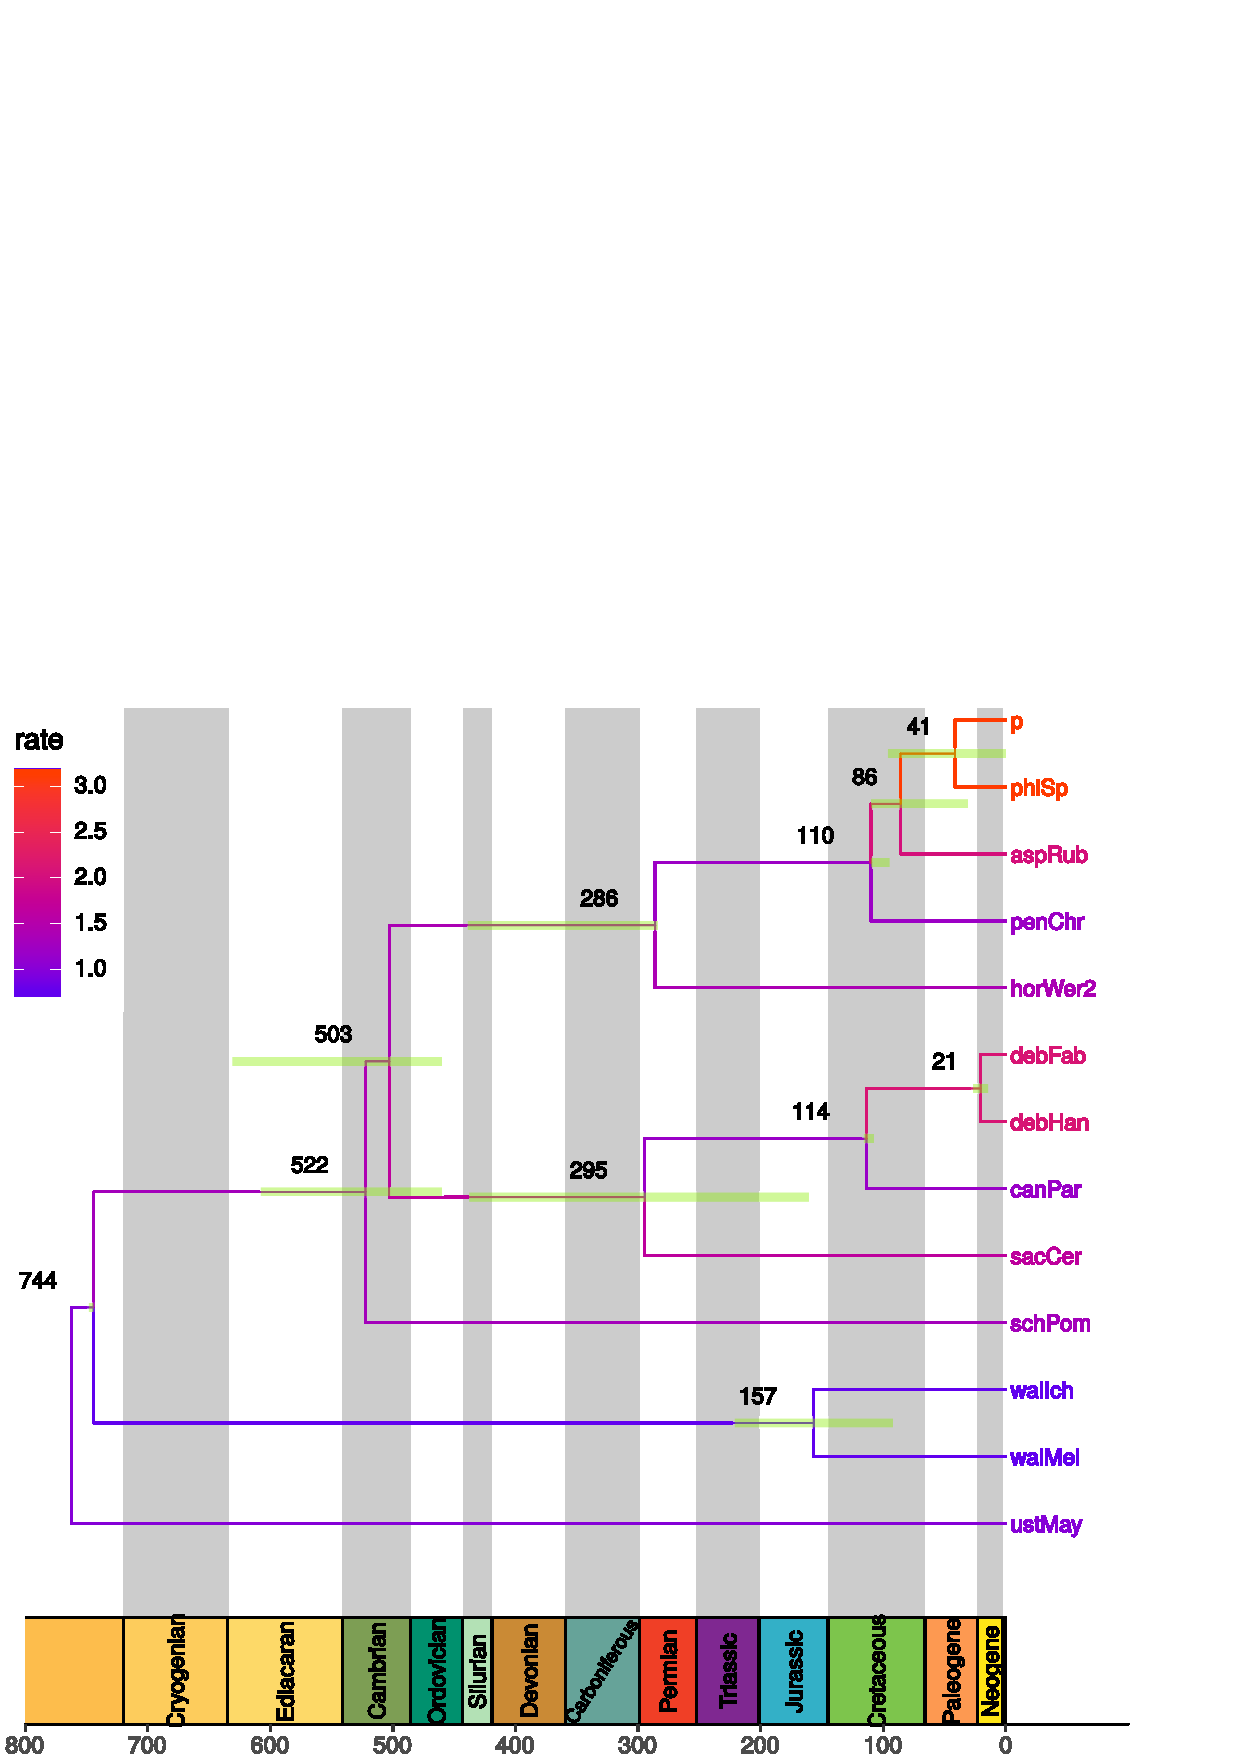
\includegraphics[width=0.9\linewidth]{./geophyloTree.pdf}
  \caption{\label{fig:gainLossTree}  Timetree analysis using the RelTime method. A timetree inferred using the Reltime method~\cite{Tamura2018, Tamura2012} and Ordinary Least Squares estimates of branch lengths. The timetree was computed using 9 calibration constraints. The proportion of sites where at least 1 unambiguous base is present in at least 1 sequence for each descendent clade is shown next to each internal node in the tree. The analysis involved 13 amino acid sequences. All positions containing gaps and missing data were eliminated. There were a total of 37607 positions in the final dataset. Evolutionary analyses were conducted in MEGA X~\cite{Kumar2018}}
\end{figure}

A timetree was constructed from the multiple sequence alignments of the proteins shared by all 13 strains and time anchors extracted from  the TimeTree database~\cite{Kumar2017}. The timetree was consistent with the currently accepted taxonomy. Based on this tree \phiSp{} and \phiScl{} separated approximately 41MYA(+/-40MYA), approximately 20MY before the split between \debFab{} and \debHan{} and 40 MY after the split between \phiSp{}, \phiScl{} and \aspRub{}. Interestingly \phiSp{} and \phiScl{} exhibit the largest evolutionary rates, followed by the two Debaryomyces species.

We used this tree to estimate the numbers of rapidly evolving annotation elements with CAFE~\cite{DeBie2006}.
We looked at the rapid evolution of families of functional annotations for the carbohydrate enzymes (Cazy)~\cite{Cantarel2009}, general enzymes from the EggNog annotation~\cite{HuertaCepas2016}, Interproscan protein domains~\cite{Jones2014a}, KEGG pathways~\cite{Ogata1999}, proteolytic enzymes (Merops)~\cite{Rawlings2014}, Pfam protein domains~\cite{Finn2014a} and transporters from TCDB~\cite{Saier2006}. The internal node with the largest numbers of rapidly evolving annotation families is the one leading to the common ancestor of \textit{Hortaea} and \textit{Aspergillus} (\textit{leotiomyceta}) (See Figure~\ref{fig:cafe}, Table~\ref{tab:cafe} and Supplementary Table 1. CAFE reports 106 IPR and 105 Pfam rapidly evolving families. The most significantly expanding families are related to fungal-specific transcription factors (p-value 4.75e-19), Cytochrome P450E (p-value 1.127e-16) and DUF3468 (p-value 1.59e-15). The branch leading to \phiSp{} exhibits the largest contraction of gene families from all species analyzed: 91 IPR, 74 Pfam, 7 Cazy, 8 tcdb 1 Merops and 8 Enzyme families contracted significantly, which is certainly linked to the 27$^\%$ decrease in genome size compared to \phiScl{}. The amino acid polyamine organocation family exhibits the largest contraction, with 8 members being lost compared to the common ancestor of \phiScl{} and \phiSp{}. Interestingly the same contraction happens in \aspRub{} where 11 family members are lost. \TODO{Discuss APC impact on halotolerance. APC downregulated in P. indica https://link.springer.com/article/10.1007$\%$2Fs11274-015-1867-5}. Other contracting transporter families are the fatty acid transporter (TCDB:4C1, -7), the iron transporter family (2A108), the amino-acid transporter family (2A18, -5), the nucleobase symporter family (2A39, -3) and the oligopeptide transporter family (2A67, -3). Another family depleted in both \phiSp{} and \aspRub{} is the  aminoglycoside phosphotransferase, a bacterial antibiotic resistance protein (IPR002575) with a loss of 15 and 13 members, respectively. 

A few annotation families showed an expansion in \phiSp{}. These families are related to the IVSP family (3A7 +9), the TRAP-C4 transporter (IPR010656 +6, PF06808 +6), the fungal cellulose binding domain (PF00734, +5), the integrase catalytic core (IPR001584), cutinase (PF01083), sodium:bile-acid symporter /arsenical resistance protein Acr3 (PF01758 +2) and secretory lipase (PF03583 +2). The increase in cellulose degrading ability due to fungal cellulose binding domain~\cite{Gilkes1991} and the cutinase~\cite{Sweigard1992} is clearly related to the wooden environment where \phiSp{} has been found. Proteins belonging to the PF01758 family confers Arsenic resistance by extrusion from cells~\cite{Fu2009}.        

\begin{figure}[htbp]
    \centering
    \includegraphics[width=0.9\linewidth]{cafeFinal.pdf}
    \caption{\label{fig:cafe} \textbf{l.h.s} Phylogenetic tree with the internal annotated with their ID and the number of families showing expansion and contraction for the annotation element KEGG, Cazy, tcdb, Enzyme and Merops. {r.h.s} Expansion and contraction counts for the tip of the tree. The color opacity is proportional to the number of contracting/expanding families. The P and M suffix stand for expansion and contraction, respectively.}
\end{figure}

\begin{table}[htbp]
\caption{\label{tab:cafe}
Table containing the number of significantly expanded and compressed family along the tree. The internal node ID corresponds to the node ID shown in Figure~\ref{fig:cafe}. Each annotation category contains the number of significantly expanding (l.h.s) and contracting families (r.h.s).}
\centering
\small
\begin{tabular}{llrrrrrrrrrrrrrr}

node & node & Cazy & Enzyme & IPR &  KEGG & Merops & Pfam & tcdb\\
\hline
<11> & I & 14 / 0 & 11 / 0 & 106 / 0 & 8 / 0 & 3 / 0 & 106 / 0 & 6 / 0\\
<13> & I & 0 / 0 & 0 / 0 & 0 / 0 & 0 / 0 & 0 / 0 & 0 & 0 / 0 / 0\\
<15> & I & 0 / 1 & 0 / 0 & 8 / 6 & 0 / 0 & 1 / 0 & 5 / 6 & 0 / 0\\
<17> & I & 0 / 0 & 0 / 0 & 8 / 1 & 0 / 0 & 0 / 0 & 6 / 1 & 0 / 0\\
<19> & I & 0 / 0 & 0 / 1 & 5 / 3 & 0 / 0 & 0 / 0 & 3 / 2 & 0 / 0\\
<1> & I & 0 / 0 & 1 / 1 & 4 / 3 & 0 / 0 & 0 / 0 & 1 / 3 & 0 / 1\\
<21> & I & 0 / 0 & 0 / 0 & 4 / 0 & 0 / 0 & 0 / 0 & 0 / 0 & 1 / 0\\
<3> & I & 0 / 0 & 0 / 0 & 0 / 0 & 0 / 0 & 0 / 0 & 0 / 0 & 0 / 0\\
<5> & I & 0 / 2 & 1 / 4 & 6 / 178 & 2 / 0 & 0 / 0 & 5 / 12 & 1 / 1\\
<7> & I & 0 / 0 & 0 / 0 & 0 / 0 & 0 / 0 & 0 / 0 & 0 / 0 & 0 / 0\\
<9> & I & 1 / 0 & 1 / 0 & 57 / 0 & 0 / 0 & 1 / 0 & 25 / 0 & 1 / 0\\
\aspRub<8> & T & 1 / 4 & 4 / 2 & 101 / 16 & 1 / 2 & 0 / 3 & 18 / 22 & 1 / 5\\
\canPar<20> & T & 0 / 0 & 0 / 1 & 14 / 5 & 0 / 0 & 1 / 1 & 6 / 7 & 1 / 0\\
\debFab<18> & T & 2 / 1 & 2 / 1 & 21 / 18 & 3 / 0 & 0 / 1 & 15 / 13 & 1 / 3\\
\debHan<16> & T & 1 / 1 & 2 / 0 & 17 / 4 & 0 / 0 & 2 / 1 & 11 / 3 & 1 / 2\\
\horWer<12> & T & 9 / 0 & 4 / 0 & 56 / 38 & 7 / 0 & 4 / 0 & 62 / 0 & 6 / 0\\
\penChr<10> & T & 10 / 0 & 4 / 0 & 179 / 1 & 3 / 1 & 4 / 0 & 80 / 2 & 7 / 0\\
\phiScl<6> & T & 9 / 1 & 10 / 2 & 65 / 5 & 6 / 0 & 3 / 1 & 77 / 6 & 8 / 2\\
\phiSp<4> & T & 0 / 7 & 1 / 8 & 4 / 91 & 0 / 6 & 1 / 1 & 6 / 74 & 2 / 8\\
\sacCer<14> & T & 3 / 0 & 2 / 0 & 16 / 3 & 1 / 0 & 1 / 0 & 12 / 10 & 1 / 0\\
\schPom<22> & T & 0 / 0 & 0 / 0 & 7 / 16 & 0 / 1 & 0 / 0 & 3 / 20 & 0 / 2\\
\ustMay<24> & T & 0 / 0 & 0 / 0 & 2 / 38 & 1 / 0 & 0 / 0 & 3 / 0 & 0 / 0\\
\walIch<2> & T & 0 / 0 & 0 / 0 & 1 / 0 & 0 / 0 & 0 / 0 & 1 / 1 & 0 / 0\\
\walMel<0> & T & 0 / 0 & 0 / 0 & 1 / 0 & 0 / 0 & 0 / 0 & 1 / 1 & 0 / 0\\
\hline
\end{tabular}
\end{table}

The over- and underrepresented annotation terms between two or more fungal genomes were alternatively studied by comparing the occurence with the help of chi-squared tests. Fungi were classified as Control (C) (\sacCer{}, \schPom{}, \ustMay{}), halophile (HH) (\walIch{}, \aspRub{}, \phiSp{}) and halotolerant (H) (\phiScl{}, \horWer2{}, \walMel{}, \penChr{}, \debFab{}, \debHan{}, \canPar{}). 
\phiSp{} compared to \phiScl{} has significantly less MFS-transporters (TCDB 2A1 2.29e-06, GO:0055085 0.0047) and aminoglycoside phosphotransferase (IPR002575 3.41e-4). With respect to \aspRub{}, \phiSp{} exhibits a depletion of MFS transporters (TCDB 2A1 0.0088, GO:0005215 1.8e-04), oxidoreductase-activity (GO:0016491 3.88e-06, GO:0016620 0.0020, GO:0016740), metal binding (GO:0008270 3.62e-12, GO:0046872 1.73e-08) and nucleotide binding (GO:0000166 7.2e-04, GO:0007264 0.0018). A similar pattern is seen when considering \phiSp{} against the other halophile fungus \walIch{}. The former is depleted in nucleotide binding, protein binding, metal binding, cell wall constituents and hydrophobin (IPR001338 1.4e-04) (See Supplementary Table and Figure~\ref{fig:ovun}). Still it is enriched in terms related to oxidation-reduction processes (GO:0005506, GO:0016705, GO:0016705), transcription factors (GO:0000981, IPR01138) and transporters (MFS, APC).
In comparison with \horWer2{}, \phiSp{} is depleted in MFS transporters but is enriched in TRAP transporter (TCDB 2A56).

\begin{figure}[htbp]
    \centering
    \includegraphics[width=0.9\linewidth]{over_under.pdf}
    \caption{\label{fig:ovun} Heatmap of the $-log(fdr)$ of the significantly enriched or depleted functional annotations {\phiSp}. 
    \textbf{A} Enriched functional terms in {\phiSp} compared to {\phiScl}, {\aspRub}, {\walIch}, the set of halophile \textit{H}, halotolerant \textit{H} and control \textit{C} fungi. Enrichment found in HH vs H, HH vs C and H vs C were also studied. \textbf{B} Depleted functional terms in {\phiSp} for the same comparisons as in \textbf{A}.}
\end{figure}

With regard to the group of salt intolerant fungi, \phiSp{} is depleted in genes involved in translation, metal ion binding, and chitinase, while it contains significantly more genes related to oxidation-reduction processes, transcription, MFS transporters and cellulose degradation. It should be noted that MFS are significantly overrepresented in the groups of halophile and halotolerant fungi when compared to the control group, but that the set of halophile fungi is depleted in MFS when compared to the class of halotolerant fungi (See Supplementary Table 1 and Figure~\cite{fig:ovun}).




The protein amino-acid composition of the C,H and HH groups for the set of ortholog genes and for the set of exported proteins was compared 
(See Figure~\ref{fig:AABIAS} and Supplementary Table 1). With regard to the control group, the conserved proteins in halophile fungi are significantly enriched in Glycine, Proline and Arginine and depleted in Isoleucine and Lysine. \TODO{Redo analysis on secreted protein}.  


%\subsection{Amino acid enrichment}

\begin{figure}
    \centering
    \includegraphics[width=0.9\linewidth]{AAAnalysis.pdf}
    caption{\label{fig:AABIAS} Bias in amino-acids distribution between the set of control, halotolerant and halophile fungi. \textbf{l.h.s} Boxplot representing the distribution AA for the 5 AA with the most significant bias between the control and halophile group  for the set of conserved(top) and secreted proteins (bottom). \textbf{r.h.s} of the $-log(fdr)$ of the significantly enriched or depleted functional annotations {\phiSp}. 
    \textbf{A} Enriched functional terms in {\phiSp} compared to {\phiScl}, {\aspRub}, {\walIch}, the set of halophile \textit{H}, halotolerant \textit{H} and control \textit{C} fungi. Enrichment found in HH vs H, HH vs C and H vs C were also studied. \textbf{B} Depleted functional terms in {\phiSp} for the same comparisons as in \textbf{A}.}
\end{figure}

\subsection{Differential expression}
In \phiScl{} 




\begin{figure}
    \centering
    \includegraphics[width=0.8\linewidth]{phiScl_SALT_summary.pdf}
    \caption{\label{fig:phiSclUpDown} Heatmap of the $-log(fdr)$ of the significantly enriched or depleted functional annotations {\phiSp}. 
    \textbf{A} Enriched functional terms in {\phiSp} compared to {\phiScl}, {\aspRub}, {\walIch}, the set of halophile \textit{H}, halotolerant \textit{H} and control \textit{C} fungi. Enrichment found in HH vs H, HH vs C and H vs C were also studied. \textbf{B} Depleted functional terms in {\phiSp} for the same comparisons as in \textbf{A}.}
\end{figure}

\begin{figure}
    \centering
    \includegraphics[width=0.8\linewidth]{phiSp_SALT_summary.pdf}
    \caption{\label{fig:phiSclUpDown} Heatmap ohttps://www.overleaf.com/project/5bcf4218dfee4857f1fc3836f the $-log(fdr)$ of the significantly enriched or depleted functional annotations {\phiSp}. 
    \textbf{A} Enriched functional terms in {\phiSp} compared to {\phiScl}, {\aspRub}, {\walIch}, the set of halophile \textit{H}, halotolerant \textit{H} and control \textit{C} fungi. Enrichment found in HH vs H, HH vs C and H vs C were also studied. \textbf{B} Depleted functional terms in {\phiSp} for the same comparisons as in \textbf{A}.}
\end{figure}

This section may be divided by subheadings. It should provide a concise and precise description of the experimental results, their interpretation as well as the experimental conclusions that can be drawn.
\begin{quote}
This section may be divided by subheadings. It should provide a concise and precise description of the experimental results, their interpretation as well as the experimental conclusions that can be drawn.
\end{quote}

%%%%%%%%%%%%%%%%%%%%%%%%%%%%%%%%%%%%%%%%%%
\subsection{Subsection}
\unskip
\subsubsection{Subsubsection}

Bulleted lists look like this:
\begin{itemize}[leftmargin=*,labelsep=5.8mm]
\item	First bullet
\item	Second bullet
\item	Third bullet
\end{itemize}

Numbered lists can be added as follows:
\begin{enumerate}[leftmargin=*,labelsep=4.9mm]
\item	First item 
\item	Second item
\item	Third item
\end{enumerate}

The text continues here.

\subsection{Figures, Tables and Schemes}

All figures and tables should be cited in the main text as Figure 1, Table 1, etc.

\begin{figure}[H]
\centering
\includegraphics[width=2 cm]{Definitions/logo-mdpi}
\caption{This is a figure, Schemes follow the same formatting. If there are multiple panels, they should be listed as: (\textbf{a}) Description of what is contained in the first panel. (\textbf{b}) Description of what is contained in the second panel. Figures should be placed in the main text near to the first time they are cited. A caption on a single line should be centered.}
\end{figure}   
 
Text

Text

\begin{table}[H]
\caption{This is a table caption. Tables should be placed in the main text near to the first time they are cited.}
\centering
%% \tablesize{} %% You can specify the fontsize here, e.g.,  \tablesize{\footnotesize}. If commented out \small will be used.
\begin{tabular}{ccc}
\toprule
\textbf{Title 1}	& \textbf{Title 2}	& \textbf{Title 3}\\
\midrule
entry 1		& data			& data\\
entry 2		& data			& data\\
\bottomrule
\end{tabular}
\end{table}

Text

Text

%\begin{listing}[H]
%\caption{Title of the listing}
%\rule{\textwidth}{1pt}
%\raggedright Text of the listing. In font size footnotesize, small, or normalsize. Preferred format: left aligned and single spaced. Preferred border format: top border line and bottom border line.
%\rule{\textwidth}{1pt}
%\end{listing}


\subsection{Formatting of Mathematical Components}

This is an example of an equation:

\begin{equation}
a + b = c
\end{equation}
%% If the documentclass option "submit" is chosen, please insert a blank line before and after any math environment (equation and eqnarray environments). This ensures correct linenumbering. The blank line should be removed when the documentclass option is changed to "accept" because the text following an equation should not be a new paragraph. 

Please punctuate equations as regular text. Theorem-type environments (including propositions, lemmas, corollaries etc.) can be formatted as follows:
%% Example of a theorem:
\begin{Theorem}
Example text of a theorem.
\end{Theorem}

The text continues here. Proofs must be formatted as follows:

%% Example of a proof:
\begin{proof}[Proof of Theorem 1]
Text of the proof. Note that the phrase `of Theorem 1' is optional if it is clear which theorem is being referred to.
\end{proof}
The text continues here.

%%%%%%%%%%%%%%%%%%%%%%%%%%%%%%%%%%%%%%%%%%
\section{Discussion}
\TODO{Discussion of \phiSp{} Figure~\ref{fig:spec} specific genes}
Authors should discuss the results and how they can be interpreted in perspective of previous studies and of the working hypotheses. The findings and their implications should be discussed in the broadest context possible. Future research directions may also be highlighted.

%%%%%%%%%%%%%%%%%%%%%%%%%%%%%%%%%%%%%%%%%%
\section{Materials and Methods}
\subsection{Cultivation}

The two examined strains \textit{Aspergillus salisburgensis} (EXF-10247/MA6005) and \textit{Aspergillus sclerotialis} (CBS 366.77/MA5985) were grown on salt yeast media (0.4 $\%$ glucose, 0.4 $\%$ yeast extract, 1.0 $\%$ malt extract, 1.2 $\%$ agar and either 5.0 $\%$ or 20.0 $\%$ NaCl). The two strains were incubated at their optimal temperature (\textit{A. salisburgensis} at room temperature,  \textit{A. sclerotialis} at  37$^{\circ}$ C) for 35 days.

\subsection{Total RNA Extraction}
After 35 days of cultivation, RNA was extracted using  FastRNA Pro RED KIT (MP Biomedicals, Santa Ana, CA, United States). For each condition and strain, 3 replicates of Total RNA were extracted following the manufactures protocol.
The quality and quantity was measured using the Agilent 2100 Bioanalyzer (Agilent Technologies, Santa Clara, CA, United States) and a Qubit 2.0 (Life Technologies, Carlsbad, CA, United States). 
\subsection{RNA library preparation}
The total RNA library was prepared as described before \cite{Poyntner2016}. mRNA was isolated from the total RNA using the Dynabeads mRNA DIRECT Micro Kit (Ambion by Life Technologies, Carlsbad, CA, United States). Subsequently the RNA library for sequencing was constructed using the Ion Total RNA-Seq kit v2 (Life Technologies, Carlsbad, CA, United States). Quality was checked using the Agilent 2100 Bioanalyzer instrument (Agilent Technologies, Santa Clara, CA, United States). The final library was size selected to 290bp using the Pippin Prep (Sage Science, Beverly, MA, United States). The following sequencing was done using the Ion Torrent Chef instrument, Ion Torrent Proton instrument and the HiQ sequencing kit (Life Technologies, Carlsbad, CA, United States). 
Materials and Methods should be described with sufficient details to allow others to replicate and build on published results. Please note that publication of your manuscript implicates that you must make all materials, data, computer code, and protocols associated with the publication available to readers. Please disclose at the submission stage any restrictions on the availability of materials or information. New methods and protocols should be described in detail while well-established methods can be briefly described and appropriately cited.

Research manuscripts reporting large datasets that are deposited in a publicly available database should specify where the data have been deposited and provide the relevant accession numbers. If the accession numbers have not yet been obtained at the time of submission, please state that they will be provided during review. They must be provided prior to publication.

Interventionary studies involving animals or humans, and other studies require ethical approval must list the authority that provided approval and the corresponding ethical approval code. 

%%%%%%%%%%%%%%%%%%%%%%%%%%%%%%%%%%%%%%%%%%
\section{Conclusions}

This section is not mandatory, but can be added to the manuscript if the discussion is unusually long or complex.

%%%%%%%%%%%%%%%%%%%%%%%%%%%%%%%%%%%%%%%%%%
\section{Patents}
This section is not mandatory, but may be added if there are patents resulting from the work reported in this manuscript.

%%%%%%%%%%%%%%%%%%%%%%%%%%%%%%%%%%%%%%%%%%
\vspace{6pt} 

%%%%%%%%%%%%%%%%%%%%%%%%%%%%%%%%%%%%%%%%%%
%% optional
%\supplementary{The following are available online at \linksupplementary{s1}, Figure S1: title, Table S1: title, Video S1: title.}

% Only for the journal Methods and Protocols:
% If you wish to submit a video article, please do so with any other supplementary material.
% \supplementary{The following are available at \linksupplementary{s1}, Figure S1: title, Table S1: title, Video S1: title. A supporting video article is available at doi: link.}

%%%%%%%%%%%%%%%%%%%%%%%%%%%%%%%%%%%%%%%%%%
\authorcontributions{For research articles with several authors, a short paragraph specifying their individual contributions must be provided. The following statements should be used “conceptualization, X.X. and Y.Y.; methodology, X.X.; software, X.X.; validation, X.X., Y.Y. and Z.Z.; formal analysis, X.X.; investigation, X.X.; resources, X.X.; data curation, X.X.; writing—original draft preparation, X.X.; writing—review and editing, X.X.; visualization, X.X.; supervision, X.X.; project administration, X.X.; funding acquisition, Y.Y.”, please turn to the  \href{http://img.mdpi.org/data/contributor-role-instruction.pdf}{CRediT taxonomy} for the term explanation. Authorship must be limited to those who have contributed substantially to the work reported.}

%%%%%%%%%%%%%%%%%%%%%%%%%%%%%%%%%%%%%%%%%%
\funding{Please add: ``This research received no external funding'' or ``This research was funded by NAME OF FUNDER grant number XXX.'' and  and ``The APC was funded by XXX''. Check carefully that the details given are accurate and use the standard spelling of funding agency names at \url{https://search.crossref.org/funding}, any errors may affect your future funding.}

%%%%%%%%%%%%%%%%%%%%%%%%%%%%%%%%%%%%%%%%%%
\acknowledgments{In this section you can acknowledge any support given which is not covered by the author contribution or funding sections. This may include administrative and technical support, or donations in kind (e.g., materials used for experiments).}

%%%%%%%%%%%%%%%%%%%%%%%%%%%%%%%%%%%%%%%%%%
\conflictsofinterest{Declare conflicts of interest or state ``The authors declare no conflict of interest.'' Authors must identify and declare any personal circumstances or interest that may be perceived as inappropriately influencing the representation or interpretation of reported research results. Any role of the funders in the design of the study; in the collection, analyses or interpretation of data; in the writing of the manuscript, or in the decision to publish the results must be declared in this section. If there is no role, please state ``The funders had no role in the design of the study; in the collection, analyses, or interpretation of data; in the writing of the manuscript, or in the decision to publish the results''.} 

%%%%%%%%%%%%%%%%%%%%%%%%%%%%%%%%%%%%%%%%%%
%% optional
\abbreviations{The following abbreviations are used in this manuscript:\\

\noindent 
\begin{tabular}{@{}ll}
MDPI & Multidisciplinary Digital Publishing Institute\\
DOAJ & Directory of open access journals\\
TLA & Three letter acronym\\
LD & linear dichroism
\end{tabular}}

%%%%%%%%%%%%%%%%%%%%%%%%%%%%%%%%%%%%%%%%%%
%% optional
\appendixtitles{no} %Leave argument "no" if all appendix headings stay EMPTY (then no dot is printed after "Appendix A"). If the appendix sections contain a heading then change the argument to "yes".
\appendixsections{multiple} %Leave argument "multiple" if there are multiple sections. Then a counter is printed ("Appendix A"). If there is only one appendix section then change the argument to "one" and no counter is printed ("Appendix").
\appendix
\section{}
\unskip
\subsection{}
The appendix is an optional section that can contain details and data supplemental to the main text. For example, explanations of experimental details that would disrupt the flow of the main text, but nonetheless remain crucial to understanding and reproducing the research shown; figures of replicates for experiments of which representative data is shown in the main text can be added here if brief, or as Supplementary data. Mathematical proofs of results not central to the paper can be added as an appendix.

\section{}
All appendix sections must be cited in the main text. In the appendixes, Figures, Tables, etc. should be labeled starting with `A', e.g., Figure A1, Figure A2, etc. 

%%%%%%%%%%%%%%%%%%%%%%%%%%%%%%%%%%%%%%%%%%
% Citations and References in Supplementary files are permitted provided that they also appear in the reference list here. 

%=====================================
% References, variant A: internal bibliography
%=====================================
\reftitle{References}
%\begin{thebibliography}{999}
% Reference 1
%\bibitem[Author1(year)]{ref-journal}
%Author1, T. The title of the cited article. {\em Journal Abbreviation} {\bf 2008}, {\em 10}, 142-149, doi:xxxxx.
% Reference 2
%\bibitem[Author2(year)]{ref-book}
%Author2, L. The title of the cited contribution. In {\em The Book Title}; Editor1, F., Editor2, A., Eds.; Publishing House: City, Country, 2007; pp. 32-58, ISBN.
%\end{thebibliography}

% The following MDPI journals use author-date citation: Arts, Econometrics, Economies, Genealogy, Humanities, IJFS, JRFM, Laws, Religions, Risks, Social Sciences. For those journals, please follow the formatting guidelines on http://www.mdpi.com/authors/references
% To cite two works by the same author: \citeauthor{ref-journal-1a} (\citeyear{ref-journal-1a}, \citeyear{ref-journal-1b}). This produces: Whittaker (1967, 1975)
% To cite two works by the same author with specific pages: \citeauthor{ref-journal-3a} (\citeyear{ref-journal-3a}, p. 328; \citeyear{ref-journal-3b}, p.475). This produces: Wong (1999, p. 328; 2000, p. 475)

%=====================================
% References, variant B: external bibliography
%=====================================
\externalbibliography{yes}
%%\bibliography{Definitions/collection}
\bibliography{Definitions/mendeleyv2}
%\addbibresource{mendeleyv2.bib}
%%%%%%%%%%%%%%%%%%%%%%%%%%%%%%%%%%%%%%%%%%
%% optional
\sampleavailability{Samples of the compounds ...... are available from the authors.}

%% for journal Sci
%\reviewreports{\\
%Reviewer 1 comments and authors’ response\\
%Reviewer 2 comments and authors’ response\\
%Reviewer 3 comments and authors’ response
%}

%%%%%%%%%%%%%%%%%%%%%%%%%%%%%%%%%%%%%%%%%%
\end{document}

